%%%%%%%%%%%%%%%%%%%%%%%%%%%%%%%%%%%%%%%%%%%%%%%
%%% DISCLAIMER: The original template for this
%%% file can be found at:
%%%
%%% https://www.overleaf.com/latex/templates/report-template-stima-laborations-overleaf-v1-dot-0/jtctxkqjnjdz 
%%%
%%% Template for lab reports for CS341 @ IITB
%%%%%%%%%%%%%%%%%%%%%%%%%%%%%%%%%%%%%%%%%%%%%%%

%%%%%%%%%%%%%%%%%%%%%%%%%%%%%% Sets the document class for the document
% Openany is added to remove the book style of starting every new chapter on an odd page (not needed for reports)
\documentclass[11pt,swedish, openany, oneside]{book}

%%%%%%%%%%%%%%%%%%%%%%%%%%%%%% Loading packages that alter the style
\usepackage[]{graphicx}
\usepackage[]{color}
\usepackage{alltt}
\usepackage[T1]{fontenc}
\usepackage[utf8]{inputenc}
%\usepackage{float}
\usepackage{floatrow}
\usepackage{subfigure}
\usepackage{multirow}
\usepackage{tablefootnote}
\usepackage{wrapfig}
\usepackage{amsmath}
\usepackage{placeins}

\usepackage{minted}

\usepackage{xcolor}

\usepackage{listings}

\setcounter{secnumdepth}{3}
\setcounter{tocdepth}{3}
\setlength{\parskip}{\smallskipamount}
% \setlength{\parindent}{0pt}

% Set page margins
\usepackage[top=90pt,bottom=80pt,left=70pt,right=70pt]{geometry}

% Package used for placeholder text
\usepackage{lipsum}

% Prevents LaTeX from filling out a page to the bottom
\raggedbottom

% Adding both languages, Swedish and English, so they can be used intermittently in for example abstracts.
\usepackage[swedish, english]{babel}

% All page numbers are positioned at the bottom of the page
\usepackage{fancyhdr}
\fancyhf{} % clear all header and footers
\fancyfoot[C]{Page \thepage}
\renewcommand{\headrulewidth}{0pt} % remove the header rule
\pagestyle{fancy}

% Changes the style of chapter headings
\usepackage{titlesec}
\titleformat{\chapter}
   {\normalfont\Large\bfseries}{\thechapter.}{1em}{}

\titleformat{\section}
   {\normalfont\large\bfseries}{\thesection}{1em}{}
% Change distance between chapter header and text
\titlespacing{\chapter}{100pt}{100pt}{3\baselineskip}

% Adds table captions above the table per default
\usepackage{float}
\floatstyle{plaintop}
\restylefloat{table}

\let\cleardoublepage\clearpage
%\let\cleardoublepage\clearemptydoublepage
%counter
\setcounter{chapter}{0}

% Adds space between caption and table
\usepackage[tableposition=top]{caption}

% Adds hyperlinks to references and ToC
\usepackage{hyperref}
\hypersetup{hidelinks,
            linkcolor = blue} % Changes the link color to black and hides the hideous red border that usually is created

% If multiple images are to be added, a folder (path) with all the images can be added here 
\graphicspath{ {images/} }

% Separates the first part of the report/thesis in Roman numerals
\frontmatter
\titlespacing{\chapter}{0pt}{0pt}{0pt}  
\titlespacing{\section}{0pt}{0pt}{0pt}  

%%%%%%%%%%%%%%%%%%%%%%%%%%%%%% Starts the document
\begin{document}

%%% Selects the language to be used for the first couple of pages
\selectlanguage{english}

%%%%% Adds the title page
\begin{titlepage}
	\clearpage\thispagestyle{empty}
	\centering
	\vspace{2cm}

	% Titles
	{\large CS490 - Autumn 2022 \par}
	\vspace{4cm}
	{\LARGE \textbf{Implementation \textit{\&} Review of \\ Persistent Memory based Applications}} \\
	\vspace{0.4cm}
	{\large \textbf{(R \textit{\&} D Report)} \par}
	\vspace{2cm}
	% ========================================================
	% If this is a team-based project, add in your team name,
	% team members along with roll numbers.
	%
	% If this is an individual project, remove the line
	% corresponding to the team name and the remaining members
	% ========================================================
	%{\normalsize {\large \textbf{Raja Gond} \texttt{(190050096)}}}\\
        {\large \texttt{Submitted By:} \texttt{Raja Gond} \texttt{(190050096)}}\\

        \vspace{1cm}
	{\large \texttt{Under the guidance of \\ Prof. Purushottam Kulkarni \textit{\&} Prof. Umesh Bellur}} 
	             % 
	             % Add more team members if there are any 
	             %
	             \par
	\vspace{1cm}
	\vfill

    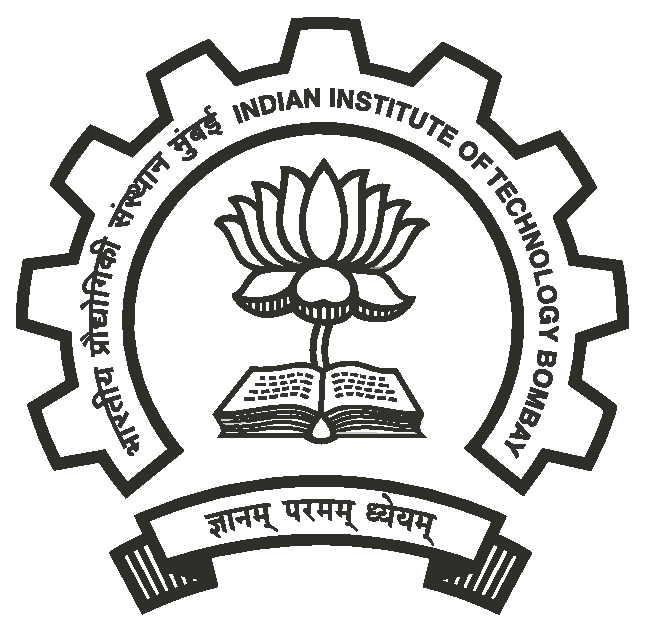
\includegraphics[scale=0.30]{iitb_logo.eps}
    
    \vspace{0.5cm}
    
	% Information about the University
	{\normalsize
		Department of Computer Science and Engineering \\
		Indian Institute of Technology Bombay  \par}
		
	% Set the date
	{\normalsize 2022-2023 \par}
	\vspace{2cm}
	
	\pagebreak

\end{titlepage}

%%%%%%%%%%%%%%%%%%%%%%%%%%%%%%%%%%%%%%%%%%%%%%%%
%% Acknowledgements
%%%%%%%%%%%%%%%%%%%%%%%%%%%%%%%%%%%%%%%%%%%%%%%%
\chapter*{\centerline{Acknowledgements}}
\addcontentsline{toc}{chapter}{\numberline{}Acknowledgements}%
\vspace{1cm}

I am grateful to Prof. Purushottam Kulkarni \textit{\&} Prof. Umesh Bellur for giving me my first taste of research. I would also like to thank them for their guidance and encouragement during the course of my project.

I would like to thank Rahul for helping me configure the optane machine.

\vspace{1cm}

Place: \texttt{Mumbai, India}    \hfill \texttt{[ Raja Gond ]}


%%%%%%%%%%%%%%%%%%%%%%%%%%%%%%%%%%%%%%%%%%%%%%%%
%% Abstract
%%%%%%%%%%%%%%%%%%%%%%%%%%%%%%%%%%%%%%%%%%%%%%%%
\chapter*{\centerline{Abstract}}
\addcontentsline{toc}{chapter}{\numberline{}Abstract}%
\vspace{1cm}

Non-volatile memory (NVM) or persistent memory (PMEM) is a new type of memory module that is capable of data persistence. Pmem provides a unique combination of affordable larger capacity. With Innovative Technology offering distinctive operating modes it adapts to your needs across workloads. It provides near-DRAM data access latency and can be directly accessed in bytes through the memory bus using CPU load. Intel Optane DC has become the first commercially available PMEM device in 2019.

Intel’s Optane Persistent Memory modules support two modes: volatile and byte-addressable persistent memory. DRAM acts as a cache for the most frequently accessed data, while Optane persistent memory provides large memory capacity. Cache management operations are handled by Intel's integrated memory controller.

We explored persistent memory in this project and did a survey of various persistent memory libraries and write the reader-writer program to understand the working of these libraries. To know how persistent memory affects large applications(such as Redis) performance we conduct performance evaluations of both pmem-redis and redis-4.0.0 using the redis benchmark.


\let\cleardoublepage\clearpage
% Adds a table of contents
\tableofcontents{}

\clearpage
%Uncomment the following three rows for a table of figures and/or tables as they are not needed for lab reports
\listoffigures
\addcontentsline{toc}{chapter}{\numberline{}List of Figures}
% \cleardoublepage\clearpage
% \listoftables
% \addcontentsline{toc}{chapter}{\numberline{}List of Tables}
\mainmatter


%%%%%%%%%%%%%%%%%%%%%%%%%%%%%%%%%%%%%%%%%%%%%%%%
%% Background
%%%%%%%%%%%%%%%%%%%%%%%%%%%%%%%%%%%%%%%%%%%%%%%%
%\chapter{Experiments}
\chapter{Life Before Persistent Memory}
Over the last few decades, computer systems have implemented the memory-storage hierarchy shown in Figure 1.1. Successive generations of technologies have iterated on the number, size, and speed of caches to ensure the CPUs have access to the most frequently used data. CPU speeds have continued to get faster, adding more cores and threads with each new CPU generation as they try to maintain Moore's Law. The capacity, price, and speed of volatile DRAM and non-volatile storage such as NAND SSDs or Hard Disk Drives have not kept pace and quickly become a bottleneck for system and application performance.\cite{pmemdoc}

\begin{figure}[H]
   \centering
   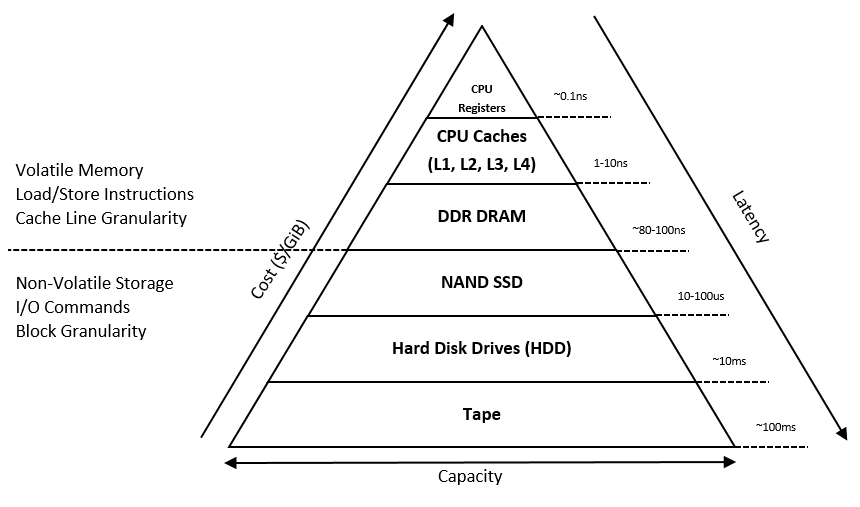
\includegraphics[width=0.6\linewidth]{lbpm1.png}
   \caption{Memory Storage Hierarchy\cite{pmemdoc}}
\end{figure}

Dynamic Random-Access Memory (\texttt{DRAM}) is a common type of random access memory (RAM) that is used in personal computers (PCs), workstations and servers. Dynamic comes from the fact that DRAM must be refreshed after a fixed time-quanta since its cells lose their state over time. DRAM is located close to a computer's processor and enables faster access to data than storage media such as hard disk drives and solid state drives but has a long access time as compared to CPU Cache and Registers.

\texttt{DRAM} is very durable and fast but not able to retain data(i.e does not provide power failure tolerance). What does this mean? If we cut off the power source(or DRAM loses its power source for any reason) the data it was processing is lost and needs to be retrieved from disk storage. This inability to retain data is known as volatility.\cite{ibm}

\textcolor{gray}{DRAM is byte addressable, and provides low latency in accessing data(as compared to pmem-more on pmem in the later section, SSDs and Hard Disks) but it is volatile and has low capacity}.

In the contrast, solid-state drives and Hard-Disk Drives(HDD) is a "non-volatile" storage drives, which means they can retain the stored data even when no power is supplied but they have low read/write speeds and have high latency when dealing with heavy workloads.  Operating systems (OS) tell the HDD to read and write data as needed by programs. The speed that the drive reads and writes this data is solely dependent on the drive itself.\cite{ibm}

\textcolor{gray}{SSD and HDD are not byte addressable and have high latency as compared to DRAM but they are cheap and non-volatile.}




%%%%%%%%%%%%%%%%%%%%%%%%%%%%%%%%%%%%%%%%%%%%%%%%%%%
%%%%%%%%% Introduction
%%%%%%%%%%%%%%%%%%%%%%%%%%%%%%%%%%%%%%%%%%%%%%%%%%
\chapter{Introduction to Persistent Memory(PMem)}
\section{Introduction - Data can't be lost, if it is on pmem}
Non-volatile memory (NVM) or persistent memory (PMEM) is a new kind of memory device that provides both near-DRAM data access latency and data persistence capability. Different from block-based devices, PMEM can be directly accessed in bytes through the memory bus using CPU load and store instruction without using block-based interfaces. Due to its high density, low cost, and near-zero standby power cost PMEM devices have been considered as a promising part of the next-generation memory hierarchy. Among all the persistent memory solutions, the Intel Optane DC Persistent Memory
(or Optane DC for short) has become the first commercially available PMEM device on the market in 2019.\cite{islam_narayanan_york_dai}

As the NVM device (e.g., Optane DC) becomes available, software developers start to consider porting their applications to persistent memory. However, to make it work efficiently, they need to have an accurate expectation of their applications performance on PMEM, as well as know how to re-design their applications to achieve the best performance.\cite{islam_narayanan_york_dai}

Persistent Memory (PMEM), also referred to as Non-Volatile Memory (NVM), or Storage Class Memory (SCM), provides a new entry in the memory-storage hierarchy shown in Figure 2.1 that fills the performance/capacity gap.\cite{pmemdoc}

\begin{figure}[H]
   \centering
   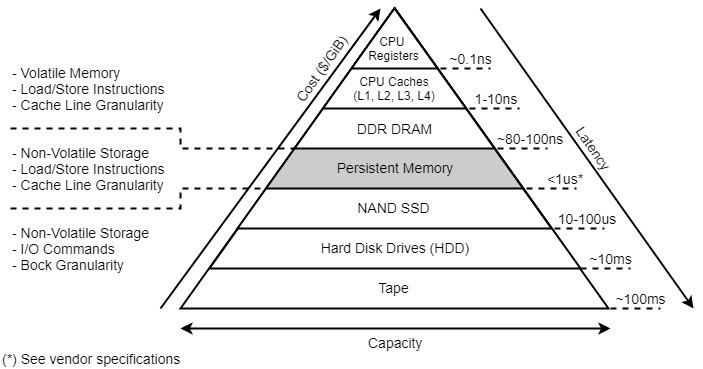
\includegraphics[width=0.6\linewidth]{itpm.png}
   \caption{Memory-Storage Hierarchy with Persistent Memory Tier\cite{pmemdoc}}
\end{figure}

With persistent memory, applications have a new tier available for data placement. In addition to the memory and storage tiers, the persistent memory tier offers greater capacity than DRAM and significantly faster performance than storage. Applications can access persistent memory like they do with traditional memory, eliminating the need to page blocks of data back and forth between memory and storage.\cite{pmemdoc}

\section{Persistent Memory Use Cases\cite{pmemuse}}
\begin{itemize}
    \item \textbf{Cloud Service Providers Cost Reduction}

    The key metric for a cloud service operator is how many VMs they can deliver to their customers, and at what cost. The size of the memory on the servers becomes the bottleneck of how many VMs they can allocate per server, limiting how low their price per VM can go. 
    
    PMem(such as Intel's Optane) is cheap compared to DRAM and  delivers a larger amount of memory per server, allocating a larger number of VMs, therefore lowering the cost per VM and increasing the competitiveness of cloud service providers.

    \item \textbf{Reliability with Large Memory Data Bases}
    
    Financial customers such as stock exchanges, banks, and mutual funds use a lot of memory databases and in-memory applications.
    \begin{itemize}
        \item \texttt{Fraud detection}
        
        Financial Institutions have very large amounts of data of transactions, customer records etc. Accessing data from disks and then performing various analytics (such as illegal transactions detection) on them is slow and time-consuming. Persistent Memory can help in improving speed.
    \end{itemize}
\end{itemize}

\section{Some new programming concerns introduced by persistent memory\cite{pmemdoc}}
It did not apply to traditional volatile memory

\begin{itemize}
    \item \texttt{Data Persistence}

    Stores are not guaranteed to be persistent until flushed.  Although this is also true for the decades-old memory-mapped file APIs (like mmap() and msync() on Linux), many programmers have not dealt with the need to flush to persistence for memory. CPUs have out-of-order CPU execution and cache access/flushing.  This means if two values are stored by the application, the order in which they become persistent may not be the order that the application wrote them.  

    \item \texttt{Data Consistency}
    
    8-byte stores are powerfail atomic on the x86 architecture -- if a powerfail happens during an aligned, 8-byte store to PMEM, either the old 8-bytes or the new 8-bytes (not a combination of the two) will be found in that location after reboot.  
    Anything larger than 8-bytes on x86 is not powerfail atomic.
    
    \item \texttt{Memory Leaks} 

    Memory leaks to persistent storage are persistent.  Rebooting the server doesn't change the on-device contents.

    \item \texttt{Byte Level Access}

    Application developers can read and write at the byte level according to the application requirements. The read/writes no longer need to be aligned or equal to storage block boundaries, eg: 512byte, 4KiB, or 8KiB.  The storage doesn't need to read an entire block to modify a few bytes, to then write that entire block back to persistent storage.  Applications are free to read/write as much or as little as required.  This improves performance and reduces memory footprint overheads.

    \item \texttt{Error Handling}

    Applications may need to detect and handle hardware errors directly. Since applications have direct access to the persistent memory media, any errors will be returned back to the application as memory errors. 
\end{itemize}


%%%%%%%%%%%%%%%%%%%%%%%%%%%%%%%%%%%%%%%
%%%% pmdk library and persistent memory programming
%%%%%%%%%%%%%%%%%%%%%%%%%%%%%%%%%%%%%%%

\chapter{Persistent Memory Programming \textit{\&} PMDK Libraries}

\section{Operating System Support for Persistent Memory}
\begin{figure}[H]
   \centering
   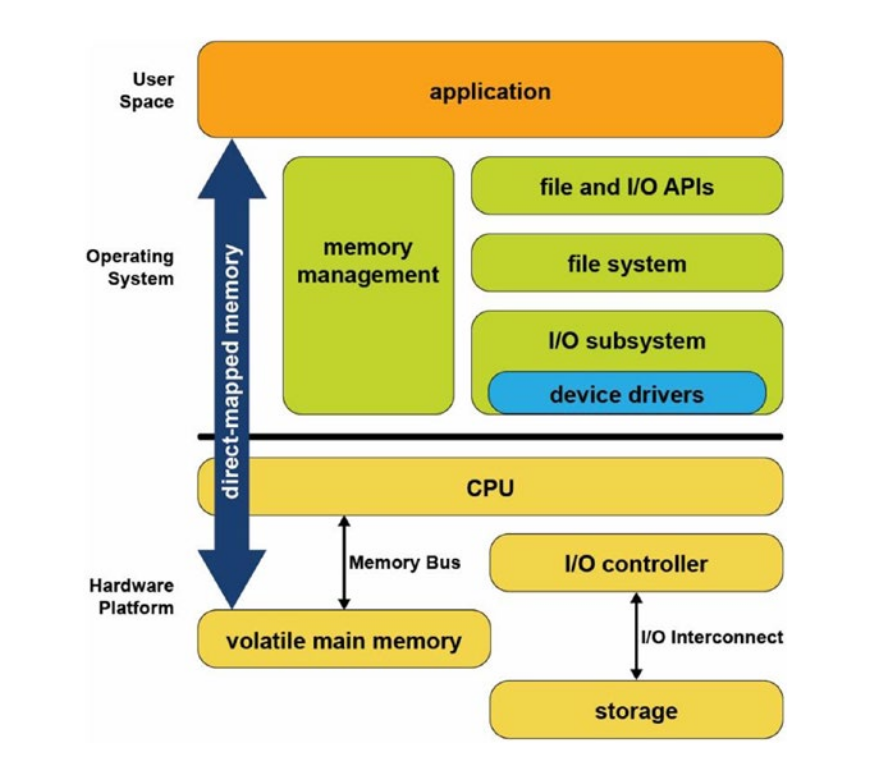
\includegraphics[width=0.6\linewidth]{oss1.png}
   \caption{Storage and volatile memory in the operating system\cite{Scargall2020}}
\end{figure}
As shown in figure 3.1, the volatile main memory is attached directly to the CPU through a memory bus. The operating system manages the mapping of memory regions directly into the application’s visible memory address space. Storage, which usually operates at speeds much slower than the CPU, is attached through an I/O controller. The operating system handles access to the storage through device driver modules loaded into the operating system's I/O subsystem.

Since persistent memory can be accessed directly by applications and can persist data in place, it allows operating systems to support a new programming model that combines the performance of memory while persisting data like a non-volatile storage device.\cite{Scargall2020}

\begin{itemize}
    \item \texttt{Persistent Memory As Block Storage}
    The first operating system extension for persistent memory is the ability to detect the existence of persistent memory modules and load a device driver into the operating system's I/O subsystem as shown in Figure 3.2. This NVDIMM driver serves two important functions. First, it provides an interface for management and system administrator utilities to configure and monitor the state of the persistent memory hardware. Second, it functions similarly to the storage device drivers.\cite{Scargall2020}
    \begin{figure}[H]
       \centering
       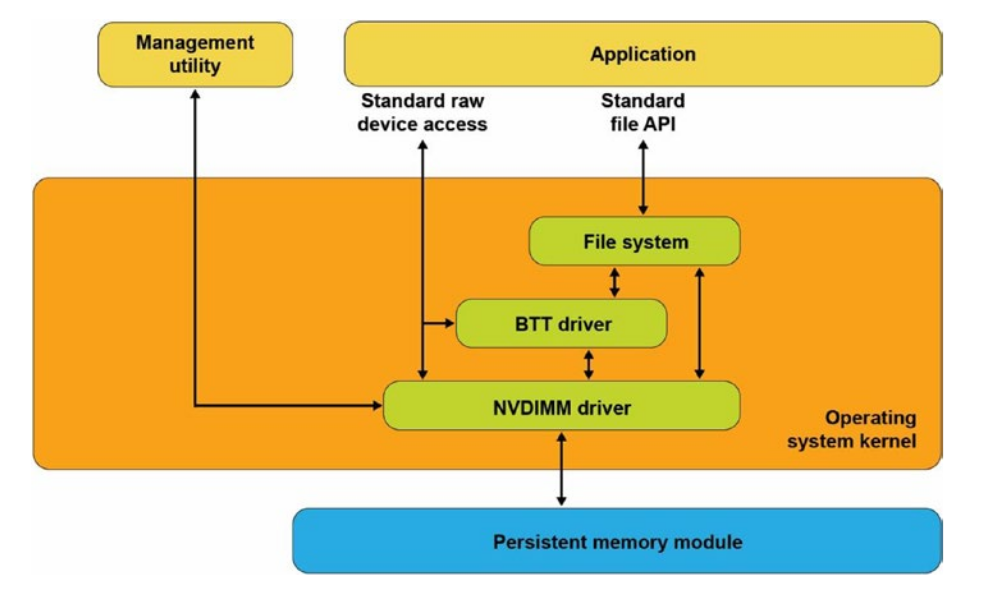
\includegraphics[width=0.6\linewidth]{oss2.png}
       \caption{Persistent Memory As Block Storage \cite{Scargall2020}}
    \end{figure}

    \item \texttt{Persistent Memory-Aware File Systems}
    \begin{figure}[H]
       \centering
       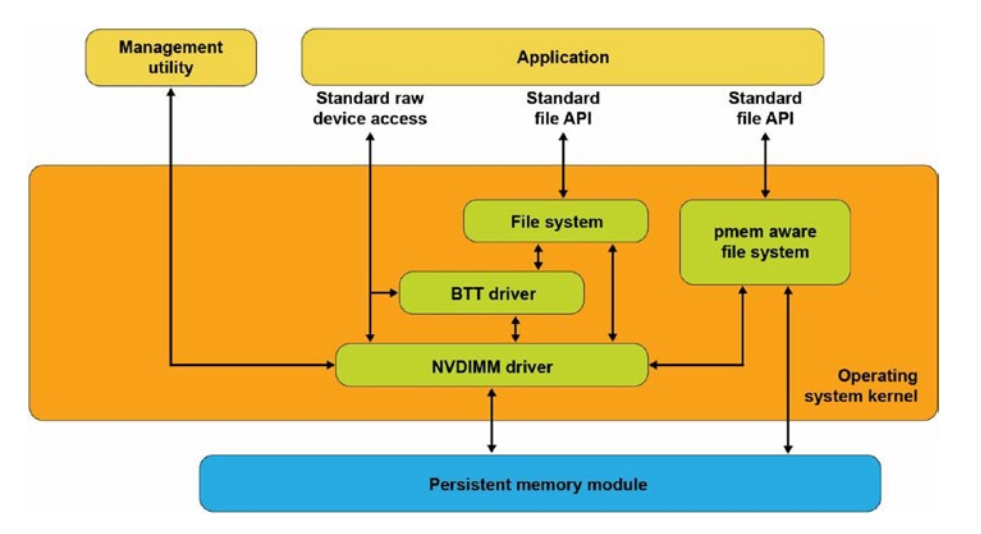
\includegraphics[width=0.6\linewidth]{oss3.png}
       \caption{Persistent Memory-Aware File Systems \cite{Scargall2020}}
    \end{figure}

    Make the operating system is to file system aware of and be optimized for persistent memory. File systems that have been extended for persistent memory include Linux ext4 and XFS, and Microsoft Windows NTFS. As shown in Figure 3.3, these file systems can either use the block driver in the I/O subsystem or bypass the I/O subsystem to directly use persistent memory as byte-addressable load/store memory as the fastest and shortest path to data stored in persistent memory.

    \item \texttt{Memory-Mapped Files}

    When memory mapping a file, the operating system adds a range to the application's virtual address space which corresponds to a range of the file, paging file data into physical memory as required. This allows an application to access and modify file data as byte-addressable in-memory data structures. This has the potential to improve performance and simplify application development, especially for applications that make frequent, small updates to file data.

        - Persistent Memory Direct Access (DAX)
    
            The persistent memory direct access feature in operating systems, referred to as DAX in Linux and Windows, uses the memory-mapped file interfaces but takes advantage of persistent memory’s native ability to both store data and to be used as memory.\cite{Scargall2020}

\end{itemize}

\subsection{Configure Intel's Optane for direct access in Linux}
Intel's Optane Persistent Memory modules support two modes: \textit{Memory Mode}, which is volatile, and \textit{App Direct mode}, which is byte-addressable persistent memory.

In Memory Mode, the DRAM acts as a cache for the most frequently accessed data, while Intel's Optane persistent memory provides large memory capacity. Cache management operations are handled by Intel's Xeon Scalable processor's integrated memory controller.

In App Direct Mode, applications and the Operating System are explicitly aware there are two types of direct load/store memory in the platform and can direct which type of data read or write is suitable for DRAM or Intel's Optane persistent memory.\cite{startguide}

\noindent Displaying persistent memory physical devices and regions on Linux

\verb|~$ sudo ipmctl show -dimm|

\noindent Displaying persistent memory physical devices, regions, and namespaces on Linux

\verb|~$ ndctl list -DRN|

\noindent Locating persistent memory on Linux

\verb|~$ df -h /dev/pmem*|

\noindent The Show Topology command displays both the PMem and DDR4 DRAM DIMMs.

\verb|~$ sudo ipmctl show -topology|

\noindent The Show Memory Resources command displays how the DDR/PMem capacity is allocated at the system level.

\verb|~$ sudo ipmctl show -memoryresources|

\noindent Create memory allocation goal

\verb|~$ sudo ipmctl create -goal PersistentMemoryType=AppDirect -y|

\noindent Create namespaces DAX support

\verb|~$ ndctl create-namespace --mode fsdax --region region0|

\noindent To get the DAX functionality, mount the file system with the dax mount option.

\verb|~$ sudo mount -o dax /dev/pmem0 /mnt/pmem/|

\section{Persistent Memory Development Kit(PMDK) Libraries\cite{pmdk, Scargall2020}}
The Persistent Memory Development Kit (PMDK) is a growing collection of libraries and tools. Tuned and validated on both Linux and Windows, the libraries build on the DAX (Direct Access) feature of those operating systems which allows applications to access persistent memory as memory-mapped files, as described in the SNIA NVM Programming Model.

The PMDK offers two library categories:
\vspace{-5pt}
\begin{enumerate}
    \item Volatile libraries are for use cases that only wish to exploit the capacity of persistent memory. Volatile libraries are typically simpler to use because they can fall back to dynamic random-access memory (DRAM) when persistent memory is not available. This provides a more straightforward implementation. Depending on the workload, they may also have lower overall overhead compared to similar persistent libraries because they do not need to ensure consistency of data in the presence of failures. for example,

    \begin{itemize}
        \item \texttt{libmemkind}

        The memkind library, called libmemkind, is a user-extensible heap manager built on top of jemalloc. The memkind library provides familiar malloc() and free() semantics.
        \item \texttt{libvmemcache}

        libvmemcache is an embeddable and lightweight in-memory caching solution that takes full advantage of large-capacity memory, such as persistent memory with direct memory access (DAX), through memory mapping in an efficient and scalable way.
    \end{itemize}
    \item Persistent libraries are for use in software that wishes to implement fail-safe persistent memory algorithms. Persistent libraries help applications maintain data structure consistency in the presence of failures.
\begin{itemize}
    \item \texttt{libpmem}
    
    libpmem is a low-level C library that provides a basic abstraction over the primitives exposed by the operating system. It automatically detects features available in the platform and chooses the right durability semantics and memory transfer (memcpy()) methods optimized for persistent memory. Most applications will need at least parts of this library.

    \item \texttt{libpmemobj}
    
    libpmemobj is a C library that provides a transactional object store, with a manual dynamic memory allocator, transactions, and general facilities for persistent memory programming. libpmemobj turns a persistent memory file into a flexible object store supporting transactions, memory management, locking, lists, and a number of other features.
    
    \item \texttt{libpmemobj-cpp}
    
    also known as libpmemobj++, is a C++ header-only library that uses the metaprogramming features of	C++ to provide a simpler, less error-prone interface to libpmemobj. It is a C++ idiomatic bindings for libpmemobj. Implementing containers from scratch will be a long effort, order of their implementation is quite important. libpmemobj++ has its  first container - an array. It is included in the pmem::obj::experimental namespace. \textit{libpmemobj++ persistent pointer} wraps around a type and provides the implementation of operator*,  operator-> and operator[]. (persistent\_ptr<>)

    \item \texttt{libpmemkv}
    
    libpmemkv is a generic embedded local key-value store optimized for persistent memory.

    \item \texttt{libpmemlog}
    
    C library that implements a persistent memory append-only log file with power fail-safe operations.

    \item \texttt{libpmemblk}
    
    C library for managing fixed-size arrays of blocks. It provides fail-safe interfaces to update the blocks through buffer-based functions.
\end{itemize}
\end{enumerate}

% {\let\clearpage\relax\chapter{Applications of Persistent Memory: PMem-Redis \textit{\&} reader-writer}}
% \section{Reader-Writer}
% Basic implementation of reader-writer using persistence memory. This program will provide power failure tolerance.\\ 
% \vspace{-5pt}
% \smash{
    \begin{minipage}[fontsize = \footnotesize]{\linewidth}
    {\let\clearpage\relax\chapter{\large Applications of Persistent Memory: PMem-Redis \textit{\&} reader-writer}}
\section{Reader-Writer}
    \paragraph{Reader-Writer using array-based approach}
    \label{lst:array_code}
    \inputminted{c}{code/arr.c}
\end{minipage}
% }

% \clearpage

% %     \hfill
% \smash{

% }
     \begin{minipage}[fontsize = \footnotesize]{\linewidth}
        \paragraph{Reader-Writer using pointer-based approach}
        \label{lst:linkedlist_code}
        \inputminted[firstline=1,lastline=39]{c++}{code/ll.cc}
    \end{minipage}
% \end{minipage}
     \begin{minipage}[fontsize = \footnotesize]{\linewidth}
        \paragraph{Reader-Writer using pointer-based approach(Cont.)}
        \label{lst:list_code}
        \inputminted[firstline=40,lastline=73]{c++}{code/ll.cc}
    \end{minipage}

The above reader-writer program is implemented with the help of pmdk libraries(more specifically, the array-based uses libpmemobj and the pointer-based program uses libpmemobj++). TX or transaction used in both programs make sure that update happens in one go. In pointer-based program, \verb|make_persistent| creates a persistent Node and \verb|delete_persistence| deletes the persistent Node. \verb|pmemobj_create| and \verb|pobj::pool<root>::create| creates the object file with given permission and size passed as arguments. \verb|file_exists| is a custom \verb|C| function that return \verb|true| if file exists.

Many APIs such as \verb|TX_ADD|, \verb|D_RO|, \verb|D_RW|, \verb|TOID| are provided by the pmdk libraries for correct implementation of the program on persistent memory. Details explanation about these APIs can be found in this \cite{Scargall2020} book.
\section{Enabling Redis for Persistent Memory: Pmem-Redis}
\subsection{Redis}
\begin{itemize}
    \item The open-source, in-memory data store implements a distributed, in-memory key value used by millions of developers as a database, cache, streaming engine, and message broker. External programs talk to Redis using a TCP socket and a Redis-specific protocol.\cite{redis}
    
    \item Redis is a data structure server. At its core, Redis provides a collection of native data types that help you solve a wide variety of problems, from caching to queuing to event processing(An event is anything that happens at a clearly defined time and that can be specifically recorded. Event processing is the process that takes events or streams of events, analyzes them and takes automatic action.)

    \item \texttt{Redis-Persistence} How Redis writes data to disk (append-only files, snapshots, etc.)?
    \begin{itemize}
        \item RDB (Redis Database): The RDB persistence performs point-in-time snapshots of your dataset at specified intervals.
        \item AOF (Append Only File): The AOF persistence logs every write operation received by the server, which will be played again at server startup, reconstructing the original dataset.
        \item No persistence: we can disable persistence completely,
        \item RDB + AOF: It is possible to combine both AOF and RDB in the same instance.
    \end{itemize} 
\end{itemize}

\subsection{Pmem-Redis}
What is Pmem-Redis\cite{pmemredis}? Pmem-Redis is one redis version that support Intel DCPMM(Data Center Persistent Memory) based on open source redis-4.0.0. It benefits the redis's performance by taking advantage of DCPMM competitive performance and persistence. Basically Pmem-Redis covers many aspects that related to DCPMM usage:
\begin{itemize}
    \item Five typical data structures optimization including: String, List, Hash, Set, Zset.
    \item  DCPMM copy-on-write
    \item  Redis LRU for DCPMM
    \item  Redis defragmentation support for DCPMM
    \item  Pointer-based redis AOF
    \item  Persistent ring buffer
\end{itemize}

\subsection{TieredMemDB}
TieredMemDB is a Redis branch that fully uses the advantages of DRAM and Intel Optane Persistent Memory (PMEM). It is fully compatible with Redis and supports all its structures and features. The main idea is to use a large PMEM capacity to store user data and DRAM speed for latency-sensitive structures. They also offer the possibility of defining the DRAM to PMEM ratio, which will be automatically monitored and maintained by the application. This allows us to fully adapt the utilization of the memory to your hardware configuration.\cite{tdb}

The source code of TieredMemDB can be found in this \href{https://github.com/TieredMemDB/TieredMemDB}{GitHub repository}.

\texttt{Features:}
\begin{itemize}
    \item Different types of memory - use both DRAM and PMEM in one application.
    \item Memory allocation policy - define how each memory should be used. You can specify DRAM / PMEM ratio that will be monitored and maintained by the application.
    \item Redis compatible - supports all features and structures of Redis.
    \item Configurable - use simple parameters to configure new features.
\end{itemize}

\section{Analysis of Pmem-Redis \textit{\&} Redis-4.0.0}
% \begin{figure}[H]
%     \centering
%     \begin{floatrow}
%         \ffigbox[0.5\textwidth]{\caption{SET: Throughput vs. number of parallel clients}}{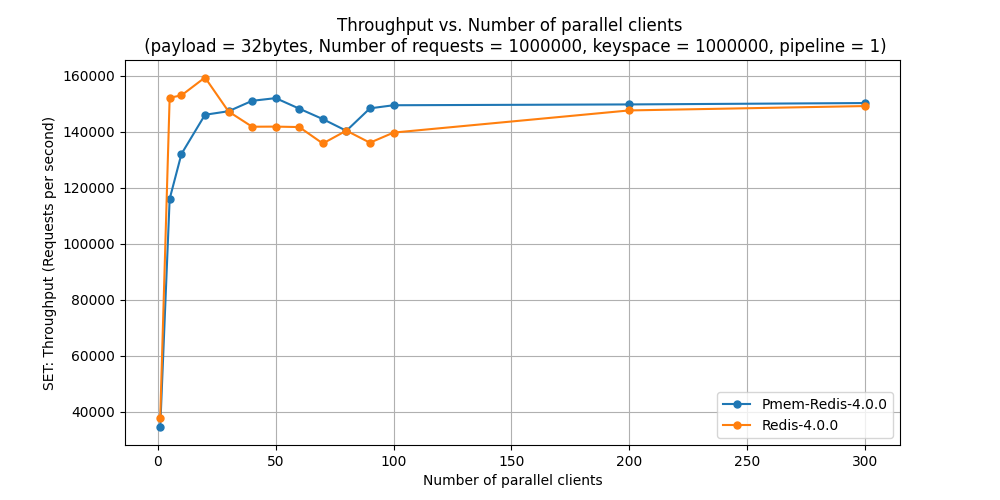
\includegraphics[width=0.5\textwidth]{pmem-redis/set1.png}}
%         %Make sure the width of the picture doesn't exceed that of the box.                                                                                                                                
%         \ffigbox[0.5\textwidth]{\caption{GET: Throughput vs. number of parallel clients}}{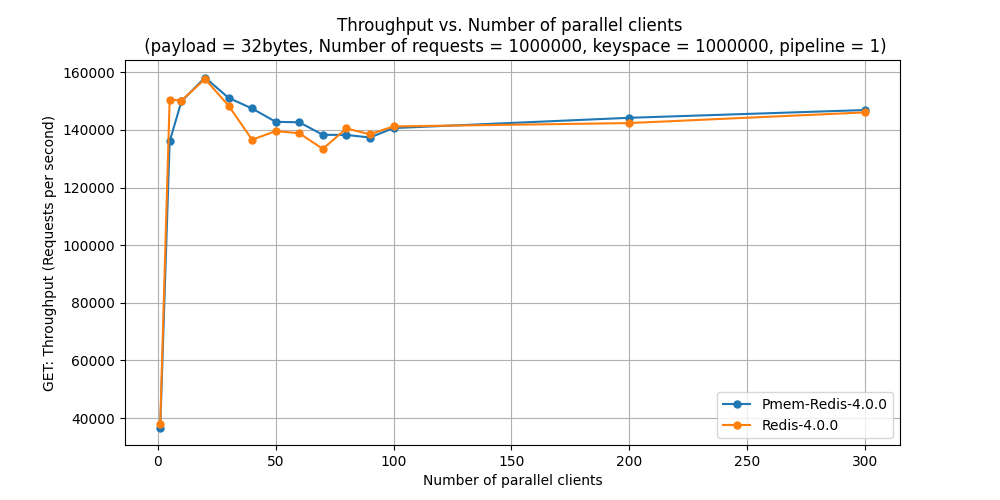
\includegraphics[width=0.5\textwidth]{pmem-redis/get1.png}}
%     \end{floatrow}
% \end{figure}

\begin{figure}[H]
    \centering
    \caption{Redis-benchmark:- SET: Throughput vs. number of parallel clients}
    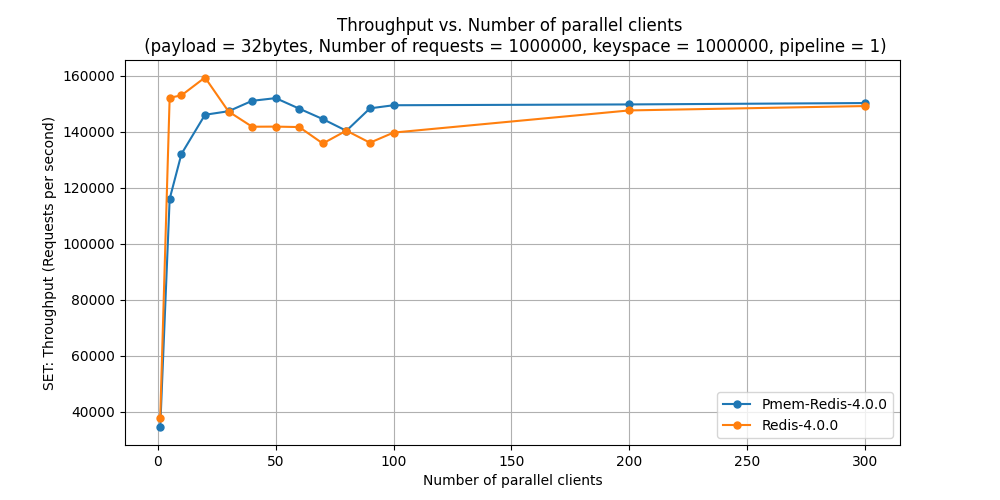
\includegraphics[width=1\textwidth]{pmem-redis/set1.png}
\end{figure}

\begin{figure}[H]
    \centering
    \caption{Redis-benchmark:- GET: Throughput vs. number of parallel clients}
    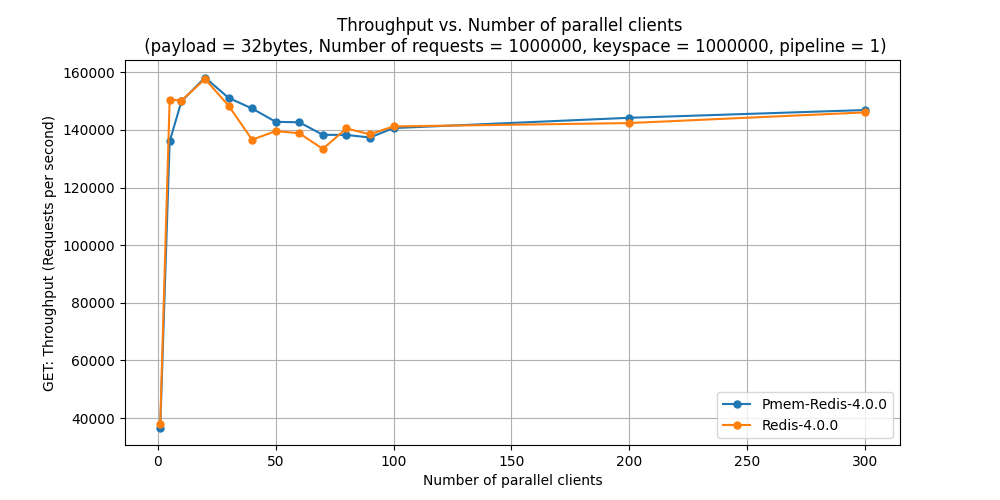
\includegraphics[width=1\textwidth]{pmem-redis/get1.png}
\end{figure}

\begin{figure}[H]
    \centering
    \caption{Redis-benchmark:- SET: Throughput vs. payload size}
    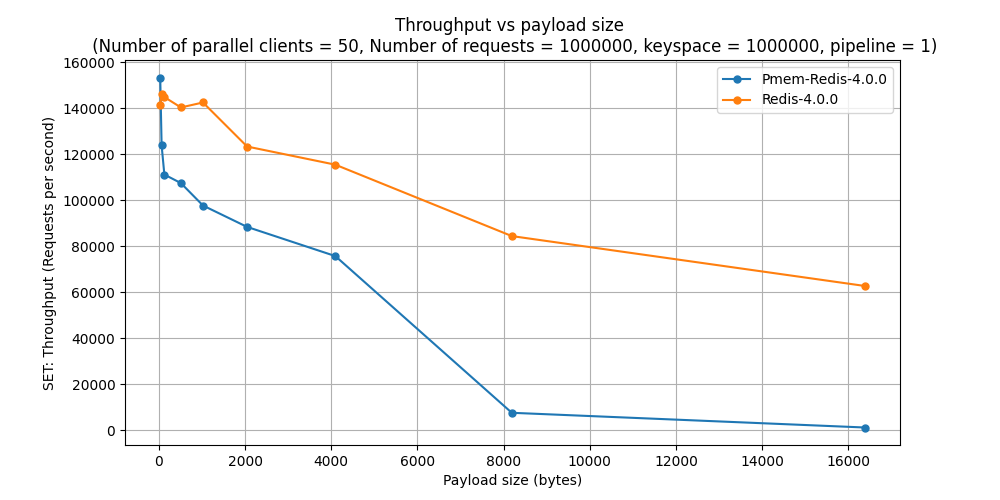
\includegraphics[width=1\textwidth]{pmem-redis/set3.png}
\end{figure}

\begin{figure}[H]
    \centering
    \caption{Redis-benchmark:- GET: Throughput vs. payload size}
    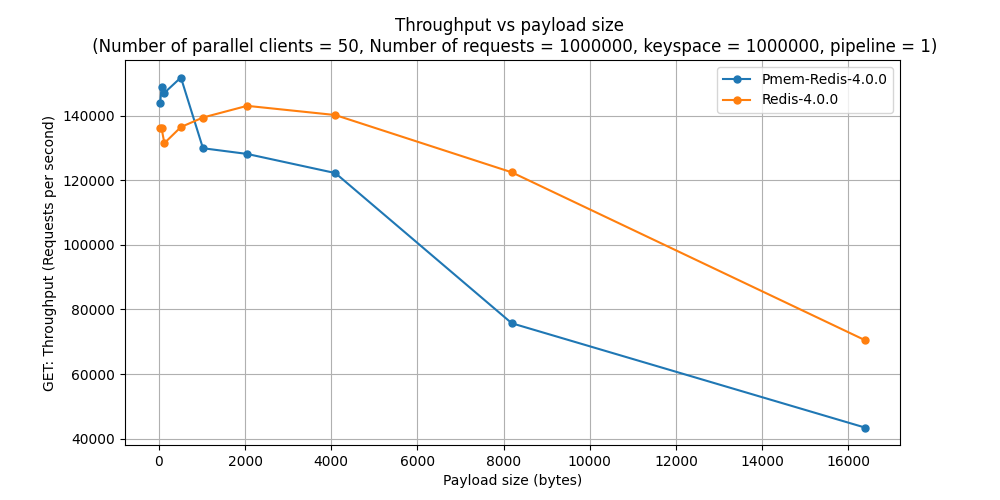
\includegraphics[width=1\textwidth]{pmem-redis/get3.png}
\end{figure}

\begin{figure}[H]
    \centering
    \caption{Redis-benchmark:- SET: Throughput vs. pipeline}
    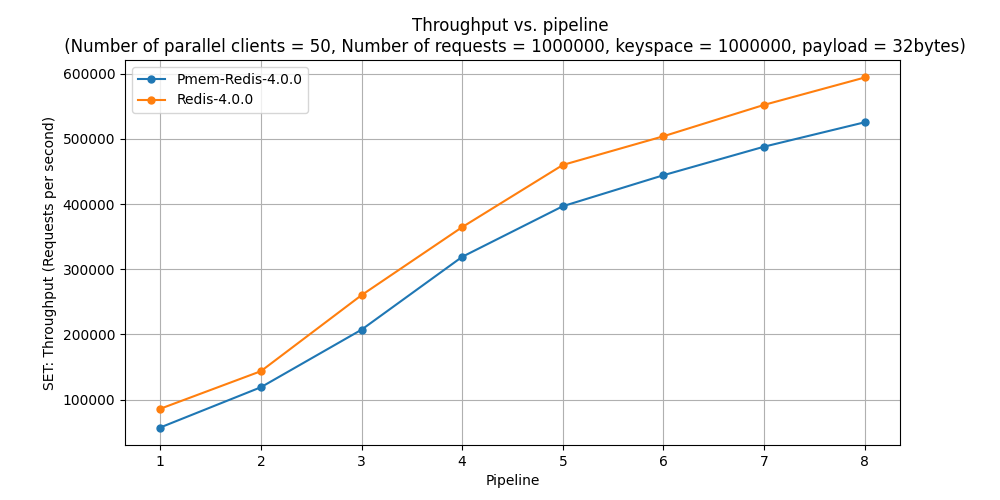
\includegraphics[width=0.9\textwidth]{pmem-redis/set2.png}
\end{figure}

\begin{figure}[H]
    \centering
    \caption{Redis-benchmark:- GET: Throughput vs. pipeline}
    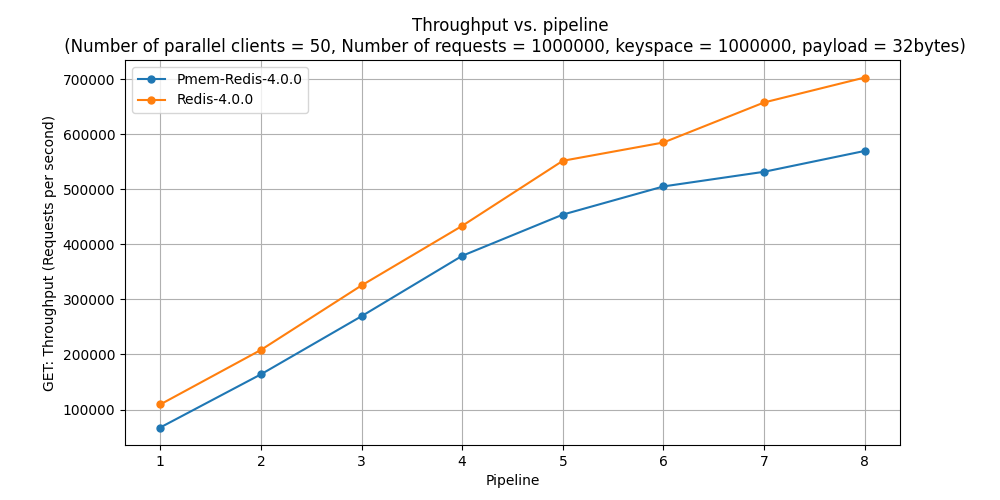
\includegraphics[width=0.9\textwidth]{pmem-redis/get2.png}
\end{figure}

I have used \href{https://redis.io/docs/management/optimization/benchmarks/#:~:text=The%20redis%2Dbenchmark%20program%20is,a%20Redis%20instance%20can%20sustain.}{redis-benchmark} and have run it on \href{https://github.com/pmem/pmem-redis}{Pmem-Redis-4.0.0} and \href{https://github.com/redis/redis/tree/4.0}{Redis-4.0.0} to record the data. On pmem-redis I have used to below command to start the redis server

\verb|sudo ./src/redis-server --nvm-maxcapacity 100 --nvm-dir /mnt/pmem --nvm-threshold 0|

The above command will start a Redis server with 100GB capacity and will use the /mnt/pmem directory as the NVM pool. The --nvm-threshold 0 option will disable the NVM threshold, which means that the server will not evict any data from NVM to DRAM.

and \verb|redis-server| to start server on Redis-4.0.0.

Both have used \textbf{jemalloc} to allocate memory(more specifically pmem-redis use \href{https://github.com/jemalloc/jemalloc/releases/tag/4.1.0}{jemalloc-4.1.0}). 

\begin{itemize}
    \item Figure 4.1 \textit{\&} Figure 4.2, both Pmem-redis-4.0.0 and redis-4.0.0 are showing almost same behaviour. Fixing payload size(data size) and the number of requests with no pipelining both are giving almost the same throughput if we vary the number of parallel clients.

    \item Figure 4.3 \textit{\&} Figure 4.4, these are the interesting plots. As we increase the payload size(data size) pmem-redis-4.0.0 goes down as compared to redis-4.0.0. For the SET case, pmem-redis-4.0.0 is poor for large payloads.
    
    \item Figure 4.5 \textit{\&} Figure 4.6, both Pmem-redis-4.0.0 and redis-4.0.0 are showing almost same behaviour(redis-4.0.0 have somewhat better throughput). Fixing payload size(data size), the number of requests and the number of clients, we can observe that redis-4.0.0 perform better if we increase pipelining.
    
\end{itemize}

\newpage

{\let\clearpage\relax\chapter{Discussions \textit{\&} Future Work}}
\vspace{1em}

Since I was not familiar with persistent memory and redis. So, I spent most of the time building
familiarity with the background material, configuring and setting up different applications (like pmem-redis, TieredmemDB) on the optane machine and trying out the basic persistent memory programming.

I plan to continue working on the project and below is the possible trajectory on which I will be working in the coming months.
\begin{itemize}
    \item Rearchitect any popular middleware that uses persistence via disks today to take advantage of persistent memory(PMem) where it exists.
    \item Exploring the specification of Compute Express Link(CXL). Compute Express Link (CXL) is an open standard for high-speed central processing unit (CPU)-to-device and CPU-to-memory connections, designed for high-performance data centre computers.
\end{itemize}

% I want to express my sincere gratitude to \texttt{Prof. Purushottam Kulkarni \textit{\&} Prof. Umesh Bellur} for the opportunity and for guiding me throughout the project.

\vspace{0.2cm}
% {\let\clearpage\relax\chapter{References}}
%\noindent \texttt{\large References}
% \begin{itemize}
%     \item \url{https://pmem.io/}
%     \item \url{https://docs.pmem.io/persistent-memory/getting-started-guide/introduction}
%     \item \url{https://github.com/Apress/programming-persistent-memory}
%     \item \url{https://github.com/efeslab/redis-pmem}
%     \item \url{https://github.com/TieredMemDB/TieredMemDB}
%     \item \url{https://github.com/jemalloc/jemalloc/releases?page=2}
%     \item \url{https://github.com/redis/redis/issues/7337}
%     \item \url{https://issues.apache.org/jira/browse/CASSANDRA-13981}
%     \item \url{https://webpages.charlotte.edu/ddai/papers/MSST20_Pmem_CameraReady.pdf}
%     \item \href{https://www.intel.com/content/www/us/en/government/podcasts/embracing-digital-transformation-episode51.html}{Practical Optane Persistent Memory Use Cases}
% \end{itemize}

\bibliographystyle{plain}
\bibliography{References.bib}
% Adds reference to the Bibliography in the ToC
% \addcontentsline{toc}{chapter}{\bibname}


\end{document}
